

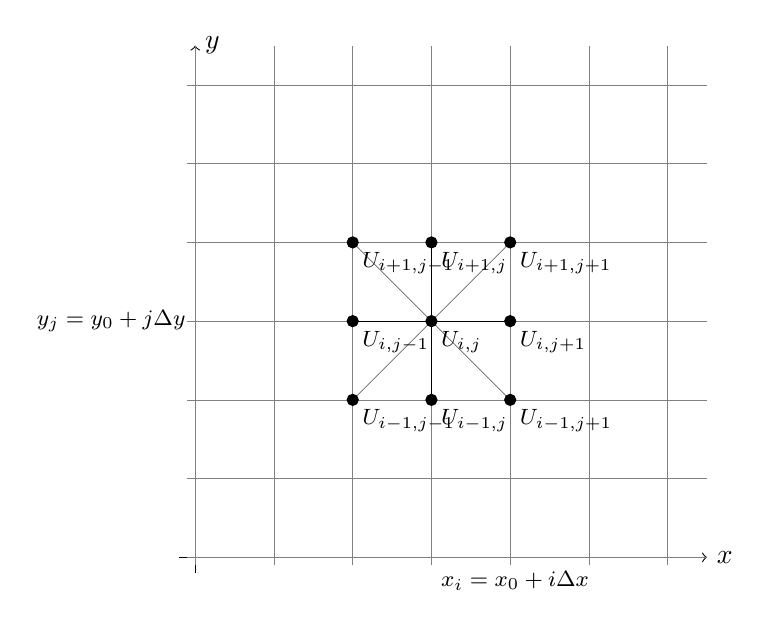
\begin{tikzpicture}
    \draw [->](0,-0.2)--(0,6.5) node[right]{$y$};
    \draw [->](-0.2,0)--(6.5,0) node[right]{$x$};
    \foreach \i in {0,...,6} {
        \draw [very thin,gray] (\i, -0.1) -- (\i,6 + 0.5);
    }
    \foreach \i in {0,...,6} {
        \draw [very thin,gray] (-0.1,\i) -- (6 + 0.5,\i);
    }
    
    \draw (3,-0.3) node[right]{\footnotesize{$x_i = x_0 + i\Delta x$}};
    \draw (0, 3) node[left]{\footnotesize{$y_j = y_0 + j\Delta y$}};
    
    \filldraw[black] (3, 3) circle (2pt) node[anchor=north west] {\footnotesize{$U_{i, j}$}};
    \filldraw[black] (2, 3) circle (2pt) node[anchor=north west] {\footnotesize{$U_{i, j-1}$}};
    \filldraw[black] (4, 3) circle (2pt) node[anchor=north west] {\footnotesize{$U_{i, j+1}$}};
    \filldraw[black] (3, 2) circle (2pt) node[anchor=north west] {\footnotesize{$U_{i-1, j}$}};
    \filldraw[black] (3, 4) circle (2pt) node[anchor=north west] {\footnotesize{$U_{i+1, j}$}};
    \filldraw[black] (4, 4) circle (2pt) node[anchor=north west] {\footnotesize{$U_{i+1, j+1}$}};
    \filldraw[black] (2, 2) circle (2pt) node[anchor=north west] {\footnotesize{$U_{i-1, j-1}$}};
    \filldraw[black] (4, 2) circle (2pt) node[anchor=north west] {\footnotesize{$U_{i-1, j+1}$}};
    \filldraw[black] (2, 4) circle (2pt) node[anchor=north west] {\footnotesize{$U_{i+1, j-1}$}};
    
    \draw [ultra thin] (3, 3) -- (2, 3);
    \draw [ultra thin] (3, 3) -- (4, 3);
    \draw [ultra thin] (3, 3) -- (3, 2);
    \draw [ultra thin] (3, 3) -- (3, 4);
    \draw [ultra thin] (3, 3) -- (4, 4);
    \draw [ultra thin] (3, 3) -- (2, 2);
    \draw [ultra thin] (3, 3) -- (4, 2);
    \draw [ultra thin] (3, 3) -- (2, 4);
    
\end{tikzpicture}